
%
\documentclass[%
 reprint,
%superscriptaddress,
%groupedaddress,
%unsortedaddress,
%runinaddress,
%frontmatterverbose, 
%preprint,
%preprintnumbers,
%nofootinbib,
%nobibnotes,
%bibnotes,
 amsmath,amssymb,
 aps,
%pra,
%prb,
%rmp,
%prstab,
%prstper,
%floatfix,
]{revtex4-2}
\usepackage{natbib}
\usepackage{graphicx}% Include figure files
\usepackage{dcolumn}% Align table columns on decimal point
\usepackage{bm}% bold math
%\usepackage{hyperref}% add hypertext capabilities
%\usepackage[mathlines]{lineno}% Enable numbering of text and display math
%\linenumbers\relax % Commence numbering lines

%\usepackage[showframe,%Uncomment any one of the following lines to test 
%%scale=0.7, marginratio={1:1, 2:3}, ignoreall,% default settings
%%text={7in,10in},centering,
%%margin=1.5in,
%%total={6.5in,8.75in}, top=1.2in, left=0.9in, includefoot,
%%height=10in,a5paper,hmargin={3cm,0.8in},
%]{geometry}

\begin{document}

%\preprint{APS/123-QED}

\title{Monte Carlo Simulation of Particle Distribution \\in Potential Wells with Thermal Reservoir }% \\


\author{Samuel Quitian Gallego$^{1}$, Ana Sofia Marulanda Duque$^{1}$}
\email{samuel.quitiang@udea.edu.co, sofia.marulanda2@udea.edu.co}
\affiliation{%
 $^1$Faculty of Natural and Exact Sciences, Physics Department, Universidad de Antioquia}

\date{\today}

\begin{abstract}
We present the implementation of a Monte Carlo-based method to explore the energy distribution of particles within an array of infinite potential wells, each containing one particle. This system is coupled to a thermal reservoir, which causes it to behave differently than if it were isolated. Our Monte Carlo simulation allows us to observe the temporal evolution of particle behavior within the potential wells, revealing how system parameters influence their dynamics, specifically the initial temperature and well size. By examining the distribution of particles across different temperatures, we gain insights into how the thermal reservoir impacts the final energy distribution and the overall equilibrium state of the system. Our results indicate that the equilibrium energy of the system increases linearly with temperature. The time required to reach the stationary state is directly proportional to the initial temperature. This project not only contributes to a deeper understanding of particle dynamics in potential wells but also highlights the importance of advanced computational methods in exploring statistical physics. 
\end{abstract}

\keywords{Metropolis, Statistical Physics}
\maketitle

%\tableofcontents

\section{\label{sec:level1}INTRODUCTION}


The study of thermal systems represents a multifaceted domain within modern physics, where the concepts of heat and temperature intertwine with the intricacies of many-body physics. While analytical solutions for systems don't consider particle interaction, such as ideal gases, the landscape becomes more challenging when interactions come into play. In these scenarios, the number of possible configurations escalates rapidly as a function of the total number of particles present. This intricate interplay makes the search for analytical solutions a  difficult task in the realm of many-body physics.

Computer simulations have evolved into necessary tools for physics research, surpassing traditional methods by offering unique perspectives and contributing significantly to theoretical understanding. In numerous cases, simulations serve as a bridge between theoretical models and experimental data, enabling direct comparisons. Among these numerical approaches, Monte Carlo simulations stand out as particularly powerful. By stochastically sampling configurations and approximating system behavior, they unveil essential insights into complex thermal systems' properties. Through simulating the dynamic interactions among particles, Monte Carlo methods provide invaluable insights into the intricate dynamics and behaviors of such systems.

In this work, we study the scenario of an array of infinite potential wells in contact with a thermal reservoir, each containing one electron. This issue arises in various fields of physics, such as condensed matter physics, quantum mechanics, statistical mechanics, and materials science \cite{shi_optical_2020} \cite{neophytou_nanostructured_2019} \cite{tsatsulnikov_modulation_1997}.
The objective of this project is to delve into the distribution of particles within the energy levels of the system upon reaching equilibrium. Additionally, it aims to explore how the system's behavior varies concerning different parameters, such as the length of the wells. To achieve this, we will use the Monte Carlo approach with the Metropolis algorithm. We aim to explore how temperature affects the final distribution of particles on energy levels, the stability of the system, and the convergence of simulation results.

\section{BACKGROUND}
\subsection{Monte Carlo- Metropolis Methods}
Monte Carlo simulations are computational methods that utilize randomness and probabilistic sampling to address problems where deterministic solutions are difficult to obtain. Despite their apparent simplicity, these methods are highly effective and widely applicable, particularly in optimization, system simulation, and data interpretation. In integral calculus, Monte Carlo simulations work by randomly generating points within a defined domain and evaluating the integrand at these points. By averaging the function values over a large number of sampled points and scaling by the domain volume, these simulations provide an estimate of the integral value. As the number of samples increases, the estimate converges to the true integral value, thanks to the law of large numbers. These methods excel in handling high-dimensional integrals, complex functions, and parameter spaces with irregular boundaries or complex geometries, making them invaluable tools in scientific research.
%--------------------------------------------------------------------
The Metropolis algorithm is widely used in statistical physics. It finds its effectiveness in stratified sampling. A difficulty with computing this with a direct random sampling of energy states (using a uniform distribution in energy) is that there may be many states that are not very likely, or have exponentially small probability.
 This can make it inconvenient to spend a lot of computational time on the contribution of these unlikely energy states.
The solution to this is achieved by generating a series of energy values consistent with a Maxwell-Boltzmann distribution to obtain an expected value for the observable of interest. \par
At its core, it utilizes Markov Chain Monte Carlo (MCMC) techniques to explore the phase space of a system and sample configurations according to their Boltzmann weights.
It generates an ordered sequence where each element in the list is derived from the previous one. Then it proceeds by proposing iterative changes to the system's configuration and accepting or rejecting these changes based on a probabilistic criterion. Specifically, it employs a detailed balance condition, ensuring that the system reaches equilibrium and samples configurations according to their equilibrium probabilities.


\subsection{Serial and Paralell Computing}
When it comes to computing, there are two main approaches: serial and parallel. In serial computing, problems are solved one instruction at a time, on one processor. This can be slow and inefficient. In parallel computing, a problem is split into smaller parts that can be tackled at the same time by multiple processors. This can save time and make computations faster \cite{rastogi_significance_nodate}. 

Parallel computing requires a way to manage the different processors and ensure they are all working on the correct part of the problem. This coordination is done through a common control mechanism \cite{rastogi_significance_nodate} .
%--------------------------------------------------------------------------
\section{METHODOLOGY}

The proposed system on this work consist on an array of infinite potential wells, each one with a fixed maximum number of energy levels $nmax=20$ that is held constant for all the simulations. The potential wells are in contact with a thermal reservoir that dictates the dynamics of the system. \par
Is considered a potential well width $l$ for all the wells and a number of particles $N$ in contact with a thermal bath at a given temperature $T$. As the system approaches stationary state, its behavior can be observed in terms of energy occupation levels distribution and average energy values.
In this case, the initial state of the system can be expressed as: 
$n_0 = (4, 3, 2, ..., 4)$
 \par
\begin{figure}[h]
    \centering
    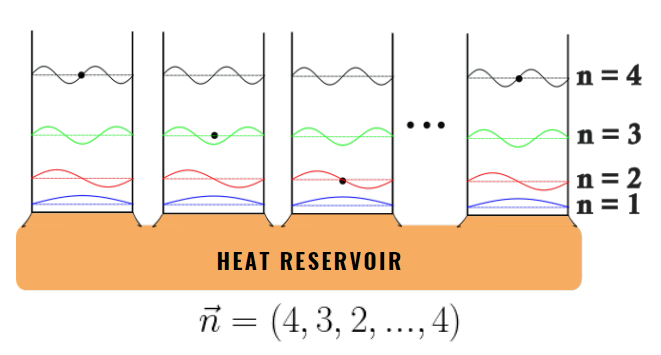
\includegraphics[width=0.4\textwidth]{reservoir.png} % Change 'example-image' to your image file name
    \caption{System of Infinite Potential Wells each one with one electron inside in a determine energy level, beneath the system scheme there is the initial vector state. }
    \label{fig:example}
\end{figure}

At its core, this project aims to investigate the distribution of particles within the energy levels of the system and explore how this behavior is affected by different parameters, such as the length of the wells. The goal is to highlight the impact of temperature on the final distribution of particles, the stability of the system, and the convergence of simulation results.


%----------------------------------------------------
\section{IMPLEMENTATION}

\subsection{The system}
It is well known that in certain physical systems, the likelihood of being in a particular state is determined by the Maxwell-Boltzmann distribution, which is a function of the energy and temperature. \par
It can be seen as the  probability $P_{s}$ that the system is in microstate $s$ with energy $E_{s}$,
\begin{equation}
        P_s=\frac{1}{Z} e^{-\beta E_s}, 
\end{equation}
where $\beta=1 / k T$ and $Z$ is the partition function. \\

The Metropolis algorithm uses acceptance ratios to determine the success of each iteration based on predetermined criteria. It iterates until the probability of each sampled state approximates the probability density of the system. This iterative process ensures that the system explores its configuration space effectively and gradually converges toward a representative sampling of states that accurately reflects the underlying distribution. By accepting or rejecting proposed moves according to the acceptance ratio, the algorithm effectively navigates through the state space, eventually providing a statistically meaningful ensemble of configurations. \\
It is possible to customize and apply this method to solve the proposed problem. The algorithm needs to rely and evaluate the transition probability, which is the change from one state to another $n_i \rightarrow n_j $. The probability of a particle of lowering down a level is due to its tendency to reach its ground state, and the probability of it ascending to a higher energy level is accounted for by $W$, which is related with the thermal energy acquire from the reservoir,

\begin{equation}
       W=P\left(n_i \rightarrow n_j\right)=\frac{p\left(E_{n_j}\right)}{p\left(E_{n_i}\right)}=\frac{e^{-\beta E_{n_j}} / Z}{e^{-\beta E_{n_i} / Z}}=e^{\beta\left(E_{n_j}-E_{n_i}\right)}.
\end{equation}

With this, the acceptance criterion can be established. The method initiates a number of random states based on the generation of sampling values, uniformly distributed. These states are then evaluated with the probability distribution and transition, subjected to the following test: 
\begin{itemize}
    \item $r: random.uniform()<0.5$: probability of downward transition
    \item $r': random.uniform()<W$ if $r>0.5$: probability of upward transition
\end{itemize}

After calculating the energy difference between transitions, the acceptance or rejection of the new transition is determined. Eventually, the system is expected to reach its stationary state, where, regardless of the initial random values generated at the start of each cycle, it maintains the same trend towards an average energy value. \par
At the end of the iterations, the particles will follow a Maxwell-Boltzmann distribution on their energy level occupancy. The Figure \ref{fig:flux} depicts the stages of the final algorithm along with its primary cycles, emphasizing the main acceptance criteria at each step.

\begin{figure}[h]
    \centering
    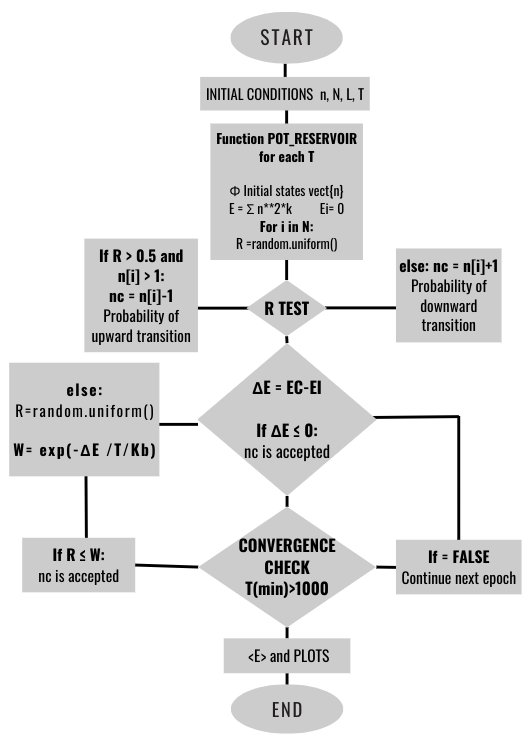
\includegraphics[width=0.5\textwidth]{diagflux.png} 
    \caption{Algorithm Flux Diagram.}
    \label{fig:flux}
\end{figure}

At its core, a $Potentialreservoir$ function is defined, taking the following inputs: 

\begin{itemize}
    \item $T (float)$: Temperature of the heat reservoir. 
    \item $N (int)$: Number of potential wells in the system.
    \item $l (float)$: Length of the wells.
    \item $nmax (int)$: Maximum level of occupancy for a well.
    \item $plot (bool)$: Whether to generate a plot of the simulation results.
    \item $live (bool)$: Whether to generate an animation of the distribution of energy states.    

\end{itemize}  

After executing the code, it yields the average energy. This enables further analysis by examining the relationship between the average energy, temperature, and well size. Such analysis allows for understanding the dependencies they have on the system's outcomes.



\section{RESULTS}
The Figure \ref{fig:T10} shows the behaviour of the system when the reservoir temperature is at $100 K$. At the beginning, the system has high energy, but after several iterations, the energy starts to decay, and eventually, it oscillates around a medium energy value. This oscillation shows minimal variation around the average value for this temperature. 

\begin{figure}[h!]
    \centering    \includegraphics[width=0.43\textwidth]{t100.png} 
    \caption{Energy evolution of an array of 20 potential wells in a thermal bath with a temperature of 100 K and a well size of 10 nm}
    \label{fig:T10}
\end{figure}

The figure \ref{fig:t1800} shows the system's behaviour when it is in contact with a thermal bath at a temperature of $2500K$. Similar to the previous case, the system starts with high energy, decreases gradually, and oscillates around a certain energy value. However, in this case, the oscillation is more significant as compared to the ones observed when the initial temperature was $100K$.
\begin{figure}[h!]
    \centering 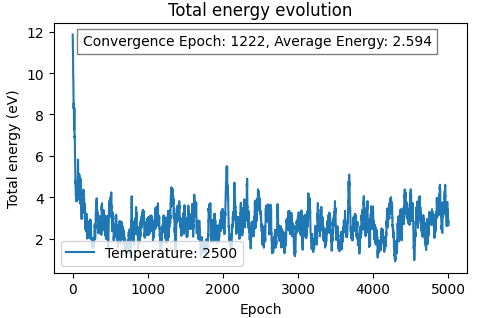
\includegraphics[width=0.42\textwidth]{T1800.png} 
    \caption{Energy evolution of an array of 20 potential wells in a thermal bath with a temperature of 2500 K and a well size of 10nm}
    \label{fig:t1800}
\end{figure}

\begin{figure}[h!]
    \centering 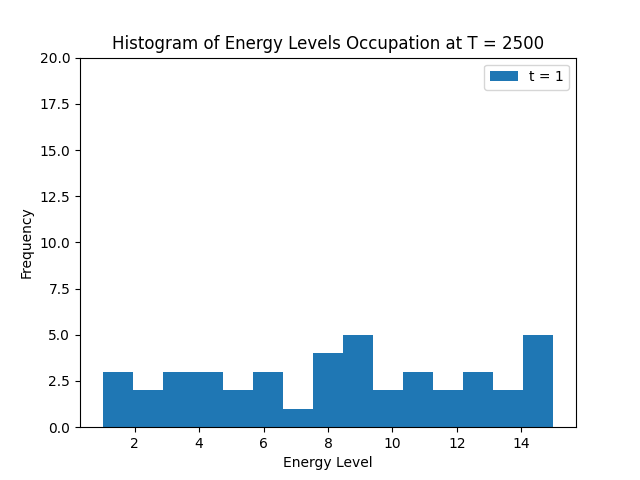
\includegraphics[width=0.41\textwidth]{Dist0.png} 
    \caption{Initial form of the energy levels occupation distribution of 50 potential wells in a thermal bath with a temperature of T = 2500 K and a well size of 10nm.}
    \label{fig:dist0}
\end{figure}

When analyzing the occupation state distribution of the system, the Figure \ref{fig:dist0} displays the initial states' occupation when the system is in contact to a thermal bath with a temperature of T = 2500 K, characterized by a uniform distribution of particles among them, in this case a larger number of potential well $N = 50$ is used in order to highlight the uniformly behaviour. However, upon reaching the equilibrium, a distinct distribution emerges, following the Maxwell-Boltzmann distribution, shown in Figure \ref{fig:distfin}. 
\begin{figure}[h]
    \centering 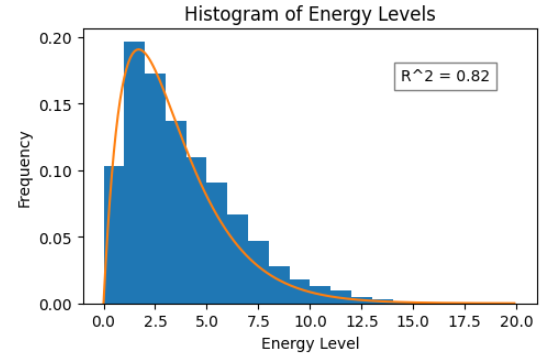
\includegraphics[width=0.41\textwidth]{ultimo.png}
    \caption{Distribution of the energy levels occupation of 20 potential wells when it reaches the thermal equilibrium with a thermal bath at a temperature of T = 2500 K and a well size of 10 nm}
    \label{fig:distfin}
\end{figure}
\par
This distribution describes the probability of finding particles at various energy levels within the system, reflecting the thermal equilibrium achieved under the specified conditions. On this case, the higher energy levels are less likely to be occupied. 
The oscillations of the system around the medium energy can be a lead into other thermal properties of the system as the variance of the energy is related to the heat capacity of the system, and can further derive in comprehending its macroscopic state and phase changes.

In order to adjust the distribution to the histogram, the ground state was redefined, instead of being n=1 was changed to n=0. 

In Figure \ref{fig:evst} is presented how the total energy of the system exhibits a linear increase with the temperature of the thermal reservoir, indicating a direct correlation between temperature and energy content. This observation follows the fundamental principle of thermodynamics, where higher temperatures lead to greater energy contributions within the system.
\begin{figure}[h!]
    \centering 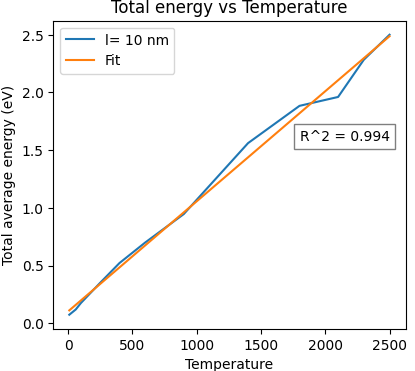
\includegraphics[width=0.31\textwidth]{TvsE.png} 
    \caption{Total average energy of the system at equilibrium respect to the temperature of the thermal bath with a well size of 10 nm. A linear function $aT+b$ is fitted with parameters a=0.00095 y b=0.10.}
    \label{fig:evst}
\end{figure}

Furthermore, the relationship between the total energy and the length of the potential well, Figure \ref{fig:svse}, reveals an inverse exponential function. This trend suggests that narrower wells result in significantly higher energy compared to wider ones, implying a sensitivity of the system's energy state to variations in well dimensions.
\begin{figure}[h!]
    \centering 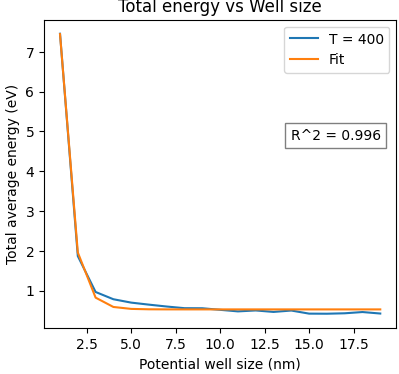
\includegraphics[width=0.32\textwidth]{EvsL.png} 
    \caption{Total average energy of the system at equilibrium respect to the well size with a thermal bath temperature of T=400 K. An exponential function $e^{-al}b+c$ is fitted with parameters a=1.57, b=33.44 and c=0.52.}
    \label{fig:svse}
\end{figure}

%-----------------------------------------------------------------------------------
\section{DISCUSSION}

\begin{itemize}
    \item \textit{Heat capacity $C_v$:} It can be computed from its energy behaviour when it is in thermal equilibrium. 
\begin{equation}
    C_v=\frac{\left\langle E^2\right\rangle - \langle E\rangle^2}{k_b T^2}
\end{equation}
Where $k_b$ is the Boltzman constant.
Expanding the discussion to include other properties of the system, particularly focusing on extracting the heat capacity from the system's evolution, was initially considered. However, the results proved to be inconclusive as they exhibited significant variability across different runs. This variability can be attributed to the inherent Markovian-stochastic nature of the problem. It is possible that inaccuracies in the calculation of the heat capacity or limitations in computing power contributed to this inconsistency. One potential avenue for addressing this issue could involve incorporating a larger number of potential wells into the model. By doing so, it is anticipated that the heat capacity would stabilize over multiple simulations, thereby facilitating more reliable estimation.
\item \textit{Quantum dots:}
One of the most intriguing systems to explore within this framework is that of quantum dots, which can be conceptualized as deliberately engineered artificial potential wells crafted within semiconductor materials. These quantum dots serve as tailored environments to confine charge carriers, such as electrons or holes, in a precise and controlled manner. Their versatility extends across a myriad of fields, including electronics, photonics, biomedical imaging, and quantum computing. Thus, a thorough understanding and meticulous study of quantum dots are imperative for enhancing their characteristics and optimizing their performance.

The results depicted in Figure \ref{fig:svse} align with the fundamental principles of photonics governing quantum dots. Notably, quantum dots exhibit light emission at higher energies when their dimensions are minimized. Consequently, the challenges elucidated in this study offer valuable insights into the behavior and optimization of quantum dots, presenting opportunities for further exploration and refinement in the realm of quantum dot research.

\end{itemize}

\section{CONCLUSIONS}

The conclusions of this study suggest paths for future research. One of them is optimizing the code and implementing advanced techniques, such as parallel programming, to generate more data and conduct a more comprehensive statistical analysis to better understand associated errors and a new try on the heat capacity calculation. This initial approach also lays the groundwork for exploring more complex systems, such as quantum dots or groups of molecules, allowing for a more precise description by interconnecting the wells and defining transition probabilities more accurately.

The implementation of the Metropolis algorithm provides an effective methodology for studying the system's energy and its relationship with input parameters, avoiding the need for complex theoretical calculations that may be intractable in certain cases. In the future, it would be interesting to compare simulation results with experimental data or theoretical predictions, providing further validation of the methodology used. Additionally, a more detailed analysis could include exploring how the system responds to different initial conditions, or instead of using random initial states, use a more fitted approach, expanding our understanding of its dynamic behavior.

Notably, the study highlights that system equilibrium is attained after several epochs, with slower convergence observed at elevated temperatures, aligning with established thermodynamic principles. Additionally, the system energy stabilizes at higher levels with increasing temperature, demonstrating a linear correlation and reinforcing the fundamental principles of statistical mechanics. These findings significantly contribute to understanding system behavior and plan ahead of new searches in this domain.



\section{REFERENCES}
\nocite{*}
%\bibliographystyle{}
\bibliography{bibliog} % Replace "references" with the name of your .bib file

\end{document}
%
